\documentclass[11pt]{article}

    \usepackage[breakable]{tcolorbox}
    \usepackage{parskip} % Stop auto-indenting (to mimic markdown behaviour)
    
    \usepackage{iftex}
    \ifPDFTeX
    	\usepackage[T1]{fontenc}
    	\usepackage{mathpazo}
    \else
    	\usepackage{fontspec}
    \fi

    % Basic figure setup, for now with no caption control since it's done
    % automatically by Pandoc (which extracts ![](path) syntax from Markdown).
    \usepackage{graphicx}
    % Maintain compatibility with old templates. Remove in nbconvert 6.0
    \let\Oldincludegraphics\includegraphics
    % Ensure that by default, figures have no caption (until we provide a
    % proper Figure object with a Caption API and a way to capture that
    % in the conversion process - todo).
    \usepackage{caption}
    \DeclareCaptionFormat{nocaption}{}
    \captionsetup{format=nocaption,aboveskip=0pt,belowskip=0pt}

    \usepackage[Export]{adjustbox} % Used to constrain images to a maximum size
    \adjustboxset{max size={0.9\linewidth}{0.9\paperheight}}
    \usepackage{float}
    \floatplacement{figure}{H} % forces figures to be placed at the correct location
    \usepackage{xcolor} % Allow colors to be defined
    \usepackage{enumerate} % Needed for markdown enumerations to work
    \usepackage{geometry} % Used to adjust the document margins
    \usepackage{amsmath} % Equations
    \usepackage{amssymb} % Equations
    \usepackage{textcomp} % defines textquotesingle
    % Hack from http://tex.stackexchange.com/a/47451/13684:
    \AtBeginDocument{%
        \def\PYZsq{\textquotesingle}% Upright quotes in Pygmentized code
    }
    \usepackage{upquote} % Upright quotes for verbatim code
    \usepackage{eurosym} % defines \euro
    \usepackage[mathletters]{ucs} % Extended unicode (utf-8) support
    \usepackage{fancyvrb} % verbatim replacement that allows latex
    \usepackage{grffile} % extends the file name processing of package graphics 
                         % to support a larger range
    \makeatletter % fix for grffile with XeLaTeX
    \def\Gread@@xetex#1{%
      \IfFileExists{"\Gin@base".bb}%
      {\Gread@eps{\Gin@base.bb}}%
      {\Gread@@xetex@aux#1}%
    }
    \makeatother

    % The hyperref package gives us a pdf with properly built
    % internal navigation ('pdf bookmarks' for the table of contents,
    % internal cross-reference links, web links for URLs, etc.)
    \usepackage{hyperref}
    % The default LaTeX title has an obnoxious amount of whitespace. By default,
    % titling removes some of it. It also provides customization options.
    \usepackage{titling}
    \usepackage{longtable} % longtable support required by pandoc >1.10
    \usepackage{booktabs}  % table support for pandoc > 1.12.2
    \usepackage[inline]{enumitem} % IRkernel/repr support (it uses the enumerate* environment)
    \usepackage[normalem]{ulem} % ulem is needed to support strikethroughs (\sout)
                                % normalem makes italics be italics, not underlines
    \usepackage{mathrsfs}
    

    
    % Colors for the hyperref package
    \definecolor{urlcolor}{rgb}{0,.145,.698}
    \definecolor{linkcolor}{rgb}{.71,0.21,0.01}
    \definecolor{citecolor}{rgb}{.12,.54,.11}

    % ANSI colors
    \definecolor{ansi-black}{HTML}{3E424D}
    \definecolor{ansi-black-intense}{HTML}{282C36}
    \definecolor{ansi-red}{HTML}{E75C58}
    \definecolor{ansi-red-intense}{HTML}{B22B31}
    \definecolor{ansi-green}{HTML}{00A250}
    \definecolor{ansi-green-intense}{HTML}{007427}
    \definecolor{ansi-yellow}{HTML}{DDB62B}
    \definecolor{ansi-yellow-intense}{HTML}{B27D12}
    \definecolor{ansi-blue}{HTML}{208FFB}
    \definecolor{ansi-blue-intense}{HTML}{0065CA}
    \definecolor{ansi-magenta}{HTML}{D160C4}
    \definecolor{ansi-magenta-intense}{HTML}{A03196}
    \definecolor{ansi-cyan}{HTML}{60C6C8}
    \definecolor{ansi-cyan-intense}{HTML}{258F8F}
    \definecolor{ansi-white}{HTML}{C5C1B4}
    \definecolor{ansi-white-intense}{HTML}{A1A6B2}
    \definecolor{ansi-default-inverse-fg}{HTML}{FFFFFF}
    \definecolor{ansi-default-inverse-bg}{HTML}{000000}

    % commands and environments needed by pandoc snippets
    % extracted from the output of `pandoc -s`
    \providecommand{\tightlist}{%
      \setlength{\itemsep}{0pt}\setlength{\parskip}{0pt}}
    \DefineVerbatimEnvironment{Highlighting}{Verbatim}{commandchars=\\\{\}}
    % Add ',fontsize=\small' for more characters per line
    \newenvironment{Shaded}{}{}
    \newcommand{\KeywordTok}[1]{\textcolor[rgb]{0.00,0.44,0.13}{\textbf{{#1}}}}
    \newcommand{\DataTypeTok}[1]{\textcolor[rgb]{0.56,0.13,0.00}{{#1}}}
    \newcommand{\DecValTok}[1]{\textcolor[rgb]{0.25,0.63,0.44}{{#1}}}
    \newcommand{\BaseNTok}[1]{\textcolor[rgb]{0.25,0.63,0.44}{{#1}}}
    \newcommand{\FloatTok}[1]{\textcolor[rgb]{0.25,0.63,0.44}{{#1}}}
    \newcommand{\CharTok}[1]{\textcolor[rgb]{0.25,0.44,0.63}{{#1}}}
    \newcommand{\StringTok}[1]{\textcolor[rgb]{0.25,0.44,0.63}{{#1}}}
    \newcommand{\CommentTok}[1]{\textcolor[rgb]{0.38,0.63,0.69}{\textit{{#1}}}}
    \newcommand{\OtherTok}[1]{\textcolor[rgb]{0.00,0.44,0.13}{{#1}}}
    \newcommand{\AlertTok}[1]{\textcolor[rgb]{1.00,0.00,0.00}{\textbf{{#1}}}}
    \newcommand{\FunctionTok}[1]{\textcolor[rgb]{0.02,0.16,0.49}{{#1}}}
    \newcommand{\RegionMarkerTok}[1]{{#1}}
    \newcommand{\ErrorTok}[1]{\textcolor[rgb]{1.00,0.00,0.00}{\textbf{{#1}}}}
    \newcommand{\NormalTok}[1]{{#1}}
    
    % Additional commands for more recent versions of Pandoc
    \newcommand{\ConstantTok}[1]{\textcolor[rgb]{0.53,0.00,0.00}{{#1}}}
    \newcommand{\SpecialCharTok}[1]{\textcolor[rgb]{0.25,0.44,0.63}{{#1}}}
    \newcommand{\VerbatimStringTok}[1]{\textcolor[rgb]{0.25,0.44,0.63}{{#1}}}
    \newcommand{\SpecialStringTok}[1]{\textcolor[rgb]{0.73,0.40,0.53}{{#1}}}
    \newcommand{\ImportTok}[1]{{#1}}
    \newcommand{\DocumentationTok}[1]{\textcolor[rgb]{0.73,0.13,0.13}{\textit{{#1}}}}
    \newcommand{\AnnotationTok}[1]{\textcolor[rgb]{0.38,0.63,0.69}{\textbf{\textit{{#1}}}}}
    \newcommand{\CommentVarTok}[1]{\textcolor[rgb]{0.38,0.63,0.69}{\textbf{\textit{{#1}}}}}
    \newcommand{\VariableTok}[1]{\textcolor[rgb]{0.10,0.09,0.49}{{#1}}}
    \newcommand{\ControlFlowTok}[1]{\textcolor[rgb]{0.00,0.44,0.13}{\textbf{{#1}}}}
    \newcommand{\OperatorTok}[1]{\textcolor[rgb]{0.40,0.40,0.40}{{#1}}}
    \newcommand{\BuiltInTok}[1]{{#1}}
    \newcommand{\ExtensionTok}[1]{{#1}}
    \newcommand{\PreprocessorTok}[1]{\textcolor[rgb]{0.74,0.48,0.00}{{#1}}}
    \newcommand{\AttributeTok}[1]{\textcolor[rgb]{0.49,0.56,0.16}{{#1}}}
    \newcommand{\InformationTok}[1]{\textcolor[rgb]{0.38,0.63,0.69}{\textbf{\textit{{#1}}}}}
    \newcommand{\WarningTok}[1]{\textcolor[rgb]{0.38,0.63,0.69}{\textbf{\textit{{#1}}}}}
    
    
    % Define a nice break command that doesn't care if a line doesn't already
    % exist.
    \def\br{\hspace*{\fill} \\* }
    % Math Jax compatibility definitions
    \def\gt{>}
    \def\lt{<}
    \let\Oldtex\TeX
    \let\Oldlatex\LaTeX
    \renewcommand{\TeX}{\textrm{\Oldtex}}
    \renewcommand{\LaTeX}{\textrm{\Oldlatex}}
    % Document parameters
    % Document title
    \title{Report}
    
    
    
    
    
% Pygments definitions
\makeatletter
\def\PY@reset{\let\PY@it=\relax \let\PY@bf=\relax%
    \let\PY@ul=\relax \let\PY@tc=\relax%
    \let\PY@bc=\relax \let\PY@ff=\relax}
\def\PY@tok#1{\csname PY@tok@#1\endcsname}
\def\PY@toks#1+{\ifx\relax#1\empty\else%
    \PY@tok{#1}\expandafter\PY@toks\fi}
\def\PY@do#1{\PY@bc{\PY@tc{\PY@ul{%
    \PY@it{\PY@bf{\PY@ff{#1}}}}}}}
\def\PY#1#2{\PY@reset\PY@toks#1+\relax+\PY@do{#2}}

\expandafter\def\csname PY@tok@w\endcsname{\def\PY@tc##1{\textcolor[rgb]{0.73,0.73,0.73}{##1}}}
\expandafter\def\csname PY@tok@c\endcsname{\let\PY@it=\textit\def\PY@tc##1{\textcolor[rgb]{0.25,0.50,0.50}{##1}}}
\expandafter\def\csname PY@tok@cp\endcsname{\def\PY@tc##1{\textcolor[rgb]{0.74,0.48,0.00}{##1}}}
\expandafter\def\csname PY@tok@k\endcsname{\let\PY@bf=\textbf\def\PY@tc##1{\textcolor[rgb]{0.00,0.50,0.00}{##1}}}
\expandafter\def\csname PY@tok@kp\endcsname{\def\PY@tc##1{\textcolor[rgb]{0.00,0.50,0.00}{##1}}}
\expandafter\def\csname PY@tok@kt\endcsname{\def\PY@tc##1{\textcolor[rgb]{0.69,0.00,0.25}{##1}}}
\expandafter\def\csname PY@tok@o\endcsname{\def\PY@tc##1{\textcolor[rgb]{0.40,0.40,0.40}{##1}}}
\expandafter\def\csname PY@tok@ow\endcsname{\let\PY@bf=\textbf\def\PY@tc##1{\textcolor[rgb]{0.67,0.13,1.00}{##1}}}
\expandafter\def\csname PY@tok@nb\endcsname{\def\PY@tc##1{\textcolor[rgb]{0.00,0.50,0.00}{##1}}}
\expandafter\def\csname PY@tok@nf\endcsname{\def\PY@tc##1{\textcolor[rgb]{0.00,0.00,1.00}{##1}}}
\expandafter\def\csname PY@tok@nc\endcsname{\let\PY@bf=\textbf\def\PY@tc##1{\textcolor[rgb]{0.00,0.00,1.00}{##1}}}
\expandafter\def\csname PY@tok@nn\endcsname{\let\PY@bf=\textbf\def\PY@tc##1{\textcolor[rgb]{0.00,0.00,1.00}{##1}}}
\expandafter\def\csname PY@tok@ne\endcsname{\let\PY@bf=\textbf\def\PY@tc##1{\textcolor[rgb]{0.82,0.25,0.23}{##1}}}
\expandafter\def\csname PY@tok@nv\endcsname{\def\PY@tc##1{\textcolor[rgb]{0.10,0.09,0.49}{##1}}}
\expandafter\def\csname PY@tok@no\endcsname{\def\PY@tc##1{\textcolor[rgb]{0.53,0.00,0.00}{##1}}}
\expandafter\def\csname PY@tok@nl\endcsname{\def\PY@tc##1{\textcolor[rgb]{0.63,0.63,0.00}{##1}}}
\expandafter\def\csname PY@tok@ni\endcsname{\let\PY@bf=\textbf\def\PY@tc##1{\textcolor[rgb]{0.60,0.60,0.60}{##1}}}
\expandafter\def\csname PY@tok@na\endcsname{\def\PY@tc##1{\textcolor[rgb]{0.49,0.56,0.16}{##1}}}
\expandafter\def\csname PY@tok@nt\endcsname{\let\PY@bf=\textbf\def\PY@tc##1{\textcolor[rgb]{0.00,0.50,0.00}{##1}}}
\expandafter\def\csname PY@tok@nd\endcsname{\def\PY@tc##1{\textcolor[rgb]{0.67,0.13,1.00}{##1}}}
\expandafter\def\csname PY@tok@s\endcsname{\def\PY@tc##1{\textcolor[rgb]{0.73,0.13,0.13}{##1}}}
\expandafter\def\csname PY@tok@sd\endcsname{\let\PY@it=\textit\def\PY@tc##1{\textcolor[rgb]{0.73,0.13,0.13}{##1}}}
\expandafter\def\csname PY@tok@si\endcsname{\let\PY@bf=\textbf\def\PY@tc##1{\textcolor[rgb]{0.73,0.40,0.53}{##1}}}
\expandafter\def\csname PY@tok@se\endcsname{\let\PY@bf=\textbf\def\PY@tc##1{\textcolor[rgb]{0.73,0.40,0.13}{##1}}}
\expandafter\def\csname PY@tok@sr\endcsname{\def\PY@tc##1{\textcolor[rgb]{0.73,0.40,0.53}{##1}}}
\expandafter\def\csname PY@tok@ss\endcsname{\def\PY@tc##1{\textcolor[rgb]{0.10,0.09,0.49}{##1}}}
\expandafter\def\csname PY@tok@sx\endcsname{\def\PY@tc##1{\textcolor[rgb]{0.00,0.50,0.00}{##1}}}
\expandafter\def\csname PY@tok@m\endcsname{\def\PY@tc##1{\textcolor[rgb]{0.40,0.40,0.40}{##1}}}
\expandafter\def\csname PY@tok@gh\endcsname{\let\PY@bf=\textbf\def\PY@tc##1{\textcolor[rgb]{0.00,0.00,0.50}{##1}}}
\expandafter\def\csname PY@tok@gu\endcsname{\let\PY@bf=\textbf\def\PY@tc##1{\textcolor[rgb]{0.50,0.00,0.50}{##1}}}
\expandafter\def\csname PY@tok@gd\endcsname{\def\PY@tc##1{\textcolor[rgb]{0.63,0.00,0.00}{##1}}}
\expandafter\def\csname PY@tok@gi\endcsname{\def\PY@tc##1{\textcolor[rgb]{0.00,0.63,0.00}{##1}}}
\expandafter\def\csname PY@tok@gr\endcsname{\def\PY@tc##1{\textcolor[rgb]{1.00,0.00,0.00}{##1}}}
\expandafter\def\csname PY@tok@ge\endcsname{\let\PY@it=\textit}
\expandafter\def\csname PY@tok@gs\endcsname{\let\PY@bf=\textbf}
\expandafter\def\csname PY@tok@gp\endcsname{\let\PY@bf=\textbf\def\PY@tc##1{\textcolor[rgb]{0.00,0.00,0.50}{##1}}}
\expandafter\def\csname PY@tok@go\endcsname{\def\PY@tc##1{\textcolor[rgb]{0.53,0.53,0.53}{##1}}}
\expandafter\def\csname PY@tok@gt\endcsname{\def\PY@tc##1{\textcolor[rgb]{0.00,0.27,0.87}{##1}}}
\expandafter\def\csname PY@tok@err\endcsname{\def\PY@bc##1{\setlength{\fboxsep}{0pt}\fcolorbox[rgb]{1.00,0.00,0.00}{1,1,1}{\strut ##1}}}
\expandafter\def\csname PY@tok@kc\endcsname{\let\PY@bf=\textbf\def\PY@tc##1{\textcolor[rgb]{0.00,0.50,0.00}{##1}}}
\expandafter\def\csname PY@tok@kd\endcsname{\let\PY@bf=\textbf\def\PY@tc##1{\textcolor[rgb]{0.00,0.50,0.00}{##1}}}
\expandafter\def\csname PY@tok@kn\endcsname{\let\PY@bf=\textbf\def\PY@tc##1{\textcolor[rgb]{0.00,0.50,0.00}{##1}}}
\expandafter\def\csname PY@tok@kr\endcsname{\let\PY@bf=\textbf\def\PY@tc##1{\textcolor[rgb]{0.00,0.50,0.00}{##1}}}
\expandafter\def\csname PY@tok@bp\endcsname{\def\PY@tc##1{\textcolor[rgb]{0.00,0.50,0.00}{##1}}}
\expandafter\def\csname PY@tok@fm\endcsname{\def\PY@tc##1{\textcolor[rgb]{0.00,0.00,1.00}{##1}}}
\expandafter\def\csname PY@tok@vc\endcsname{\def\PY@tc##1{\textcolor[rgb]{0.10,0.09,0.49}{##1}}}
\expandafter\def\csname PY@tok@vg\endcsname{\def\PY@tc##1{\textcolor[rgb]{0.10,0.09,0.49}{##1}}}
\expandafter\def\csname PY@tok@vi\endcsname{\def\PY@tc##1{\textcolor[rgb]{0.10,0.09,0.49}{##1}}}
\expandafter\def\csname PY@tok@vm\endcsname{\def\PY@tc##1{\textcolor[rgb]{0.10,0.09,0.49}{##1}}}
\expandafter\def\csname PY@tok@sa\endcsname{\def\PY@tc##1{\textcolor[rgb]{0.73,0.13,0.13}{##1}}}
\expandafter\def\csname PY@tok@sb\endcsname{\def\PY@tc##1{\textcolor[rgb]{0.73,0.13,0.13}{##1}}}
\expandafter\def\csname PY@tok@sc\endcsname{\def\PY@tc##1{\textcolor[rgb]{0.73,0.13,0.13}{##1}}}
\expandafter\def\csname PY@tok@dl\endcsname{\def\PY@tc##1{\textcolor[rgb]{0.73,0.13,0.13}{##1}}}
\expandafter\def\csname PY@tok@s2\endcsname{\def\PY@tc##1{\textcolor[rgb]{0.73,0.13,0.13}{##1}}}
\expandafter\def\csname PY@tok@sh\endcsname{\def\PY@tc##1{\textcolor[rgb]{0.73,0.13,0.13}{##1}}}
\expandafter\def\csname PY@tok@s1\endcsname{\def\PY@tc##1{\textcolor[rgb]{0.73,0.13,0.13}{##1}}}
\expandafter\def\csname PY@tok@mb\endcsname{\def\PY@tc##1{\textcolor[rgb]{0.40,0.40,0.40}{##1}}}
\expandafter\def\csname PY@tok@mf\endcsname{\def\PY@tc##1{\textcolor[rgb]{0.40,0.40,0.40}{##1}}}
\expandafter\def\csname PY@tok@mh\endcsname{\def\PY@tc##1{\textcolor[rgb]{0.40,0.40,0.40}{##1}}}
\expandafter\def\csname PY@tok@mi\endcsname{\def\PY@tc##1{\textcolor[rgb]{0.40,0.40,0.40}{##1}}}
\expandafter\def\csname PY@tok@il\endcsname{\def\PY@tc##1{\textcolor[rgb]{0.40,0.40,0.40}{##1}}}
\expandafter\def\csname PY@tok@mo\endcsname{\def\PY@tc##1{\textcolor[rgb]{0.40,0.40,0.40}{##1}}}
\expandafter\def\csname PY@tok@ch\endcsname{\let\PY@it=\textit\def\PY@tc##1{\textcolor[rgb]{0.25,0.50,0.50}{##1}}}
\expandafter\def\csname PY@tok@cm\endcsname{\let\PY@it=\textit\def\PY@tc##1{\textcolor[rgb]{0.25,0.50,0.50}{##1}}}
\expandafter\def\csname PY@tok@cpf\endcsname{\let\PY@it=\textit\def\PY@tc##1{\textcolor[rgb]{0.25,0.50,0.50}{##1}}}
\expandafter\def\csname PY@tok@c1\endcsname{\let\PY@it=\textit\def\PY@tc##1{\textcolor[rgb]{0.25,0.50,0.50}{##1}}}
\expandafter\def\csname PY@tok@cs\endcsname{\let\PY@it=\textit\def\PY@tc##1{\textcolor[rgb]{0.25,0.50,0.50}{##1}}}

\def\PYZbs{\char`\\}
\def\PYZus{\char`\_}
\def\PYZob{\char`\{}
\def\PYZcb{\char`\}}
\def\PYZca{\char`\^}
\def\PYZam{\char`\&}
\def\PYZlt{\char`\<}
\def\PYZgt{\char`\>}
\def\PYZsh{\char`\#}
\def\PYZpc{\char`\%}
\def\PYZdl{\char`\$}
\def\PYZhy{\char`\-}
\def\PYZsq{\char`\'}
\def\PYZdq{\char`\"}
\def\PYZti{\char`\~}
% for compatibility with earlier versions
\def\PYZat{@}
\def\PYZlb{[}
\def\PYZrb{]}
\makeatother


    % For linebreaks inside Verbatim environment from package fancyvrb. 
    \makeatletter
        \newbox\Wrappedcontinuationbox 
        \newbox\Wrappedvisiblespacebox 
        \newcommand*\Wrappedvisiblespace {\textcolor{red}{\textvisiblespace}} 
        \newcommand*\Wrappedcontinuationsymbol {\textcolor{red}{\llap{\tiny$\m@th\hookrightarrow$}}} 
        \newcommand*\Wrappedcontinuationindent {3ex } 
        \newcommand*\Wrappedafterbreak {\kern\Wrappedcontinuationindent\copy\Wrappedcontinuationbox} 
        % Take advantage of the already applied Pygments mark-up to insert 
        % potential linebreaks for TeX processing. 
        %        {, <, #, %, $, ' and ": go to next line. 
        %        _, }, ^, &, >, - and ~: stay at end of broken line. 
        % Use of \textquotesingle for straight quote. 
        \newcommand*\Wrappedbreaksatspecials {% 
            \def\PYGZus{\discretionary{\char`\_}{\Wrappedafterbreak}{\char`\_}}% 
            \def\PYGZob{\discretionary{}{\Wrappedafterbreak\char`\{}{\char`\{}}% 
            \def\PYGZcb{\discretionary{\char`\}}{\Wrappedafterbreak}{\char`\}}}% 
            \def\PYGZca{\discretionary{\char`\^}{\Wrappedafterbreak}{\char`\^}}% 
            \def\PYGZam{\discretionary{\char`\&}{\Wrappedafterbreak}{\char`\&}}% 
            \def\PYGZlt{\discretionary{}{\Wrappedafterbreak\char`\<}{\char`\<}}% 
            \def\PYGZgt{\discretionary{\char`\>}{\Wrappedafterbreak}{\char`\>}}% 
            \def\PYGZsh{\discretionary{}{\Wrappedafterbreak\char`\#}{\char`\#}}% 
            \def\PYGZpc{\discretionary{}{\Wrappedafterbreak\char`\%}{\char`\%}}% 
            \def\PYGZdl{\discretionary{}{\Wrappedafterbreak\char`\$}{\char`\$}}% 
            \def\PYGZhy{\discretionary{\char`\-}{\Wrappedafterbreak}{\char`\-}}% 
            \def\PYGZsq{\discretionary{}{\Wrappedafterbreak\textquotesingle}{\textquotesingle}}% 
            \def\PYGZdq{\discretionary{}{\Wrappedafterbreak\char`\"}{\char`\"}}% 
            \def\PYGZti{\discretionary{\char`\~}{\Wrappedafterbreak}{\char`\~}}% 
        } 
        % Some characters . , ; ? ! / are not pygmentized. 
        % This macro makes them "active" and they will insert potential linebreaks 
        \newcommand*\Wrappedbreaksatpunct {% 
            \lccode`\~`\.\lowercase{\def~}{\discretionary{\hbox{\char`\.}}{\Wrappedafterbreak}{\hbox{\char`\.}}}% 
            \lccode`\~`\,\lowercase{\def~}{\discretionary{\hbox{\char`\,}}{\Wrappedafterbreak}{\hbox{\char`\,}}}% 
            \lccode`\~`\;\lowercase{\def~}{\discretionary{\hbox{\char`\;}}{\Wrappedafterbreak}{\hbox{\char`\;}}}% 
            \lccode`\~`\:\lowercase{\def~}{\discretionary{\hbox{\char`\:}}{\Wrappedafterbreak}{\hbox{\char`\:}}}% 
            \lccode`\~`\?\lowercase{\def~}{\discretionary{\hbox{\char`\?}}{\Wrappedafterbreak}{\hbox{\char`\?}}}% 
            \lccode`\~`\!\lowercase{\def~}{\discretionary{\hbox{\char`\!}}{\Wrappedafterbreak}{\hbox{\char`\!}}}% 
            \lccode`\~`\/\lowercase{\def~}{\discretionary{\hbox{\char`\/}}{\Wrappedafterbreak}{\hbox{\char`\/}}}% 
            \catcode`\.\active
            \catcode`\,\active 
            \catcode`\;\active
            \catcode`\:\active
            \catcode`\?\active
            \catcode`\!\active
            \catcode`\/\active 
            \lccode`\~`\~ 	
        }
    \makeatother

    \let\OriginalVerbatim=\Verbatim
    \makeatletter
    \renewcommand{\Verbatim}[1][1]{%
        %\parskip\z@skip
        \sbox\Wrappedcontinuationbox {\Wrappedcontinuationsymbol}%
        \sbox\Wrappedvisiblespacebox {\FV@SetupFont\Wrappedvisiblespace}%
        \def\FancyVerbFormatLine ##1{\hsize\linewidth
            \vtop{\raggedright\hyphenpenalty\z@\exhyphenpenalty\z@
                \doublehyphendemerits\z@\finalhyphendemerits\z@
                \strut ##1\strut}%
        }%
        % If the linebreak is at a space, the latter will be displayed as visible
        % space at end of first line, and a continuation symbol starts next line.
        % Stretch/shrink are however usually zero for typewriter font.
        \def\FV@Space {%
            \nobreak\hskip\z@ plus\fontdimen3\font minus\fontdimen4\font
            \discretionary{\copy\Wrappedvisiblespacebox}{\Wrappedafterbreak}
            {\kern\fontdimen2\font}%
        }%
        
        % Allow breaks at special characters using \PYG... macros.
        \Wrappedbreaksatspecials
        % Breaks at punctuation characters . , ; ? ! and / need catcode=\active 	
        \OriginalVerbatim[#1,codes*=\Wrappedbreaksatpunct]%
    }
    \makeatother

    % Exact colors from NB
    \definecolor{incolor}{HTML}{303F9F}
    \definecolor{outcolor}{HTML}{D84315}
    \definecolor{cellborder}{HTML}{CFCFCF}
    \definecolor{cellbackground}{HTML}{F7F7F7}
    
    % prompt
    \makeatletter
    \newcommand{\boxspacing}{\kern\kvtcb@left@rule\kern\kvtcb@boxsep}
    \makeatother
    \newcommand{\prompt}[4]{
        \ttfamily\llap{{\color{#2}[#3]:\hspace{3pt}#4}}\vspace{-\baselineskip}
    }
    

    
    % Prevent overflowing lines due to hard-to-break entities
    \sloppy 
    % Setup hyperref package
    \hypersetup{
      breaklinks=true,  % so long urls are correctly broken across lines
      colorlinks=true,
      urlcolor=urlcolor,
      linkcolor=linkcolor,
      citecolor=citecolor,
      }
    % Slightly bigger margins than the latex defaults
    
    \geometry{verbose,tmargin=1in,bmargin=1in,lmargin=1in,rmargin=1in}
    
    

\begin{document}
    
    \maketitle
    
    

    
    \hypertarget{school-of-engineering-and-applied-science-seas-ahmedabad-university}{%
\section{School of Engineering and Applied Science (SEAS), Ahmedabad
University}\label{school-of-engineering-and-applied-science-seas-ahmedabad-university}}

\hypertarget{b.techict-semester-iv-probability-and-random-processes-mat-202}{%
\section{B.Tech(ICT) Semester IV: Probability and Random Processes (MAT
202)}\label{b.techict-semester-iv-probability-and-random-processes-mat-202}}

\begin{itemize}
\tightlist
\item
  Group No : S\_M1
\item
  Kaushal Patil (AU1841040), Arpitsingh Vaghela(AU1841034)
\item
  Project Title : Modelling probabilistic fatigue crack propogation data
  and predicting model parameters
\end{itemize}

\hypertarget{introduction}{%
\subsection{1 Introduction}\label{introduction}}

\hypertarget{background}{%
\subsubsection{1.1 Background}\label{background}}

Mechanical modelling tends to be a very complex mathematical task.One of
the most important problems realted to modelling probability in
mechanics is to find the reliabity of materials that are used to build
objects. A lot of research has taken place to compute fatigue effects on
materials and structures.There have been a lot of developments in this
area after the proposal Paris' Law. Most of the models proposed realted
to fatigue crack propogation are deterministic and have some limitations
such as that they arise from arbitary empirical assumptions.A proper
estimation of fatigue crack porpogation rates with respect to residual
stress and stress ratio helps us to estimate optimal materials for
mechanical tasks. For e.g. : To determine the type of steel to be used
when we are building a bridge. Proper estimation of fatigue crack
proporgation and finding its probabilisitic curves also gives great
insights to the propertiees of material and can be useful when the
material is being improved, i.e.~at the time of development on newer
types of alloys.

The First breakthrough in the field of fatigue propogation estimation
was the Paris' Law which was followed by various
approaches{[}3{]}.Initially Local strain-based approches were proposed
to model fatigue crack propogation on notch based components further a
link was established between local strain-based approached to fatigue
and Frature mechanics based fatigue crack propogation
models.{[}1,5-10{]} As research continued models were proposed that
using residual stress concepts ecplained stress ratio effects as well as
interaction effects on crack growth rates.Several approches were
proposed which were analytical and or numerical.{[}11-14{]}The
underlying concept behind the proposed local approaches for fatigue
crack propagation modelling consists of assuming fatigue crack
propagation as a process of continuous failure of consecutive
representative material elements (continuous re-initializations). Such a
kind of approaches has been demonstrated to correlate fatigue crack
propagation data from several sources, including the stress ratio
effects{[}10-14{]}. The crack tip stress-strain fields are computed
using elastoplastic analysis, which are applied together a fatigue
damage law to predict the failure of the representative material
elements. The simplified method of Neuber{[}15{]} or Moftakhar{[}16{]}
et al.~may be used to compute the elastoplastic stress field at the
crack tip vicinity using the elastic stress distribution given by the
Fracture Mechanics.{[}1,16-17{]} One Such model (given by
Noorzi){[}1,10-11{]} the unigrow model, modelled the fatigue crack
growth based on elastic--plastic crack tip stress--strain history
regarded the process of fatigue crack propogation as a process of
successive crack re-initiation in the crack tip region. {[}1{]}{[}0{]}

We take the unigrow model and extend it to relate it with a
probabilistic contruct to find probabilistic fatigue crack propagation
rates various materials. The Unigrow model to derive probabilistic
fatigue crack propogation \$ da/dN-\bigtriangleup K \$ fields for a
particular selected material ((S355) structural mild steel){[}0{]}, for
distinct stress ratios.The Deterministic model uses Morrows equation,
Strain life relation along with the SWT relation to model parameters
deterministically.For Probabilistic approach the strain-life field
proposed by Castillo and Fernandez-Canteli {[}20{]} and
Shane-Watson-Topper-life field {[}0{]} which are based on Weibull
Distribution are used to generalize the results to account for mean
stress effects using percentile curves. The simulation was modelled
using the data acquired{[}19,0{]} and was further extended where we
tried to make a prediction model for Threshold value of life
time{[}N0{]}, Endurance limit of strain {[}E0{]}, Fatigue Limit of SWT
parameter{[}SWT{]} and the Weibull
parameters(lambda(Position),delta(Scale),Beta(Shape)) by Running Batch
Gradient Descent{[}Reference to ML Glossary{]} on Loss function from
{[}27{]} and further using probability-weighted moments from {[}27{]} to
predict N0,E0,SWT and Weibull parameters. The Probabilistic Life time
fields are combined with Unigrow model {[}0-1{]} to finally compute the
probabilistic fatigue crack proppogation field for distinct stress
ratios.

\hypertarget{motivation}{%
\subsubsection{1.2 Motivation}\label{motivation}}

The current deterministic works take into account a lot of parameters
and some of these parameters cannot be determined easily or at all and
hence these works take arbitary assumptions in the process of modelling.
To solve this (Our Base Article) proposes a probabilistic model that not
only arises from sound statistical and physical assumtions, it also
manages to provide a probabilistic definiton of the whole strain-life
field. Further, since mechanical modelling is a complex task and takes
into account a lot of parameters, we have tried to simplify the process
of finding probabilistic fatigue crack propogation fields.Not only this
we have tried to use Gradient Descent Regression and
Probability-weighted moments method to estimate certain parameters
required for the task.

\hypertarget{problem-statement-case-study}{%
\subsubsection{1.3 Problem Statement/ Case
Study}\label{problem-statement-case-study}}

\begin{itemize}
\tightlist
\item
  To determine probabilistic fields of fatigue crack propogation rates
  wrt residual stress and stress ratio.

  \begin{itemize}
  \tightlist
  \item
    Perfomance metric : how closely the computed probabilistic field
    data and plots matches the computed data and plots given in the base
    article
  \end{itemize}
\item
  To propose a probabilistic Shane-Watson-Topper Field using the
  mathematical modelling of the Strain-Life Field proposed by
  Cantelli{[}20{]}.

  \begin{itemize}
  \tightlist
  \item
    Performance metric : how closely the shape of p-SWT-n curve match
    the experimental/deteriminstic data at a given parameter value
    (probability)
  \end{itemize}
\end{itemize}

\hypertarget{data-acusition}{%
\subsection{2 Data Acusition}\label{data-acusition}}

\begin{itemize}
\tightlist
\item
  Yes, this Special Assignment is Data Dependent.
\item
  We have gathered data from Two Types of sources:

  \begin{itemize}
  \tightlist
  \item
    Data Mentioned in reference papers {[}0,19{]}.
  \item
    Data synthesised from using simple linear equations to model plots
    of datasets given in paper using theortical formulaes supplied.

    \begin{itemize}
    \tightlist
    \item
      Postulated experimental data has been synthesised in such a way
    \end{itemize}
  \end{itemize}
\end{itemize}

\hypertarget{probabilistic-model-used-prp-concept-used}{%
\subsection{3 Probabilistic Model Used/ PRP Concept
Used}\label{probabilistic-model-used-prp-concept-used}}

We extend the Unigrow Model for Fatigue crack propogation using
probabilistic fields and work on the following model represented by:

\begin{figure}
\centering
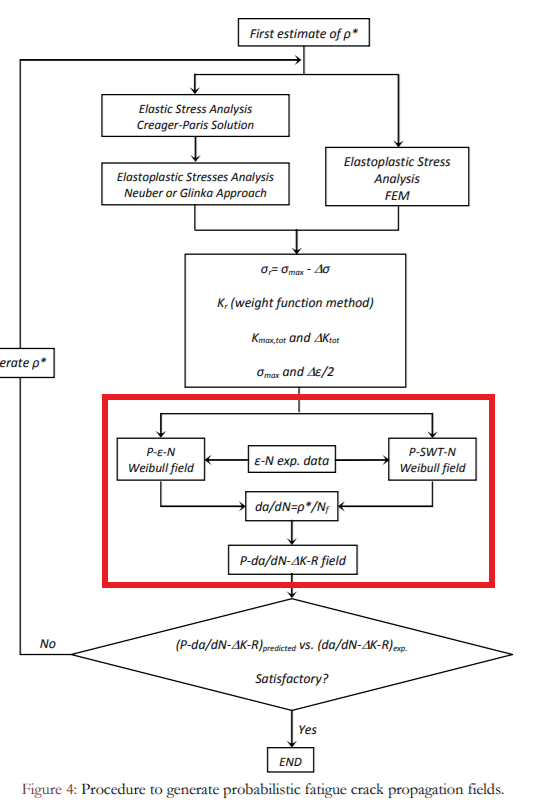
\includegraphics{BlockDiagram.png}
\caption{Block Diagram}
\end{figure}

The fatigue crack propagation modelling based on local approaches
requires a fatigue damage relation to compute the number of cycles to
fail the elementary material blocks.

Here Our main focus(Highlighted in red bounding box) is to model the
generation of probabilistic Strain-Life and SWT-Life fields. The model
assumes that the fatigue life, \(N_f\), and the total strain amplitude,
\(Ea\), are random variables.

If \(X\) is a random variable denoting the \emph{time to failure}, the
\textbf{Weibull distribution} gives a distribution for which the
\emph{failure rate} is proportional to a power of time.

\[
f_X(x) = 
\frac{\beta}{\delta}(\frac{x-\lambda}{\delta})^{\beta-1}e^{-(\frac{x-\lambda}{\delta})^\beta}
\] \[
F_X(x;\lambda,\delta,\sigma) = 1-e^{-({\frac{x-\lambda}{\delta}})^\beta}
\]

where \(\beta > 0\) is the \textbf{shape parameter},

\(\delta > 0\) is the \textbf{scale parameter},

\(\lambda > x\) is the \textbf{location parameter} (the minimum value of
X).

Percentile points,

\[
x_p = \lambda + \delta(-log(1-p))^{\frac{1}{\beta}}
\] where \(0\leq p\leq 1\)

\textbf{Important Properties of Weibull Distribution}

\begin{itemize}
\item
  Stable with respect to location and scale \[
  X \sim W(\lambda,\delta,\beta) \iff \frac{X-a}{b} \sim W(\frac{\lambda-a}{b},\frac{\delta}{b},\beta)
  \]
\item
  It is stable with respect to Minimum Operations.i.e., if
  \(X_1,X_2,X_3,.....X_m\) are independent and identical
  distribution,then \[
  X_i\sim W(\lambda,\delta,\beta) \iff min(X_1,X_2,....,X_m) \sim W(\lambda,\delta m^{\frac{1}{\beta}},\beta)
  \] if a set of independent and identical distribution is weibull then
  its minimum is also a Weibull Random Variable --- \#\#\#\# Relevant
  Variable involved for modeling: --- \(P\):Probability of fatigue
  faliure \(N\):Number of stress cycles to failure \(N_0\):Threshold
  value of N (min lifetime) \(Ea\): Strain \(Ea_0\): Endurance limit of
  Ea; \(SWT\):Smith,Watson and Topper fatigue damage parameter
  \(SWT_0\):Fatigue limit
\end{itemize}

Putting Related variables together we have three varaibles(based on II
Theorem) \#\#\#\#\# For Strain Life Field \[
\frac{N}{N_0},\frac{Ea}{Ea_0},P \\
P = q(\frac{N}{N_0},\frac{Ea}{Ea_0})
\] where \(q()\) is a function we are to determine so P can be any
monotone function of \(\frac{N}{N_0},\frac{Ea}{Ea_0}\) , as
\(h(\frac{N}{N_0})\) \(\&\) \(g(\frac{Ea}{Ea_0})\)

We denote them as \[
N^* = h(\frac{N}{N_0}) \\
SWT^* = g(\frac{Ea}{Ea_0})
\]

\hypertarget{for-swt-life-field}{%
\subparagraph{For SWT Life Field}\label{for-swt-life-field}}

\[
\frac{N}{N_0},\frac{SWT}{SWT_0},P \\
P = q(\frac{N}{N_0},\frac{SWT}{SWT_0})
\] where \(q()\) is a function we are to determine so P can be any
monotone function of \(\frac{N}{N_0},\frac{SWT}{SWT_0}\) , as
\(h(\frac{N}{N_0})\) \(\&\) \(g(\frac{SWT}{SWT_0})\)

We denote them as \[
N^* = h(\frac{N}{N_0}) \\
SWT^* = g(\frac{SWT}{SWT_0})
\]

\hypertarget{strain-life-field}{%
\subparagraph{Strain-Life Field}\label{strain-life-field}}

\[
p = F(N^*_f;E^*_a) = 1 - exp(-(\frac{log\frac{N_f}{N_0}log\frac{Ea}{Ea_0}-\lambda}{\delta})^\beta)
\]

here \(log(\frac{N_f}{N_0})loglog\frac{Ea}{Ea_0} \geq \lambda\)

p is the probability of failure, N0 and εa0 are normalizing values, and
λ, δ and β are the non-dimensional Weibull model parameters.

\[
N^*Ea^* \sim W(\lambda,\delta,\beta) \\
N^*_f\sim W(\frac{\lambda}{Ea^* },\frac{\delta}{Ea^* },\beta) \\
\]

\hypertarget{proposed-swt-n-or-s-n-field}{%
\subparagraph{Proposed SWT-N or S-N
Field}\label{proposed-swt-n-or-s-n-field}}

We have proposed SWT field as it has advantages over the normal strain
life field as it uses the SWT fatigue damage parameter.Using this Damage
Parameter we can account for mean stress effects on fatigue life
prediction.

\[
p = F(N^*_f;E^*_a) = 1 - exp(-(\frac{log\frac{N_f}{N_0}log\frac{SWT}{SWT_0}-\lambda}{\delta})^\beta)
\]

here \(log(\frac{N_f}{N_0})loglog\frac{SWT}{SWT_0} \geq \lambda\)

p is the probability of failure, N0 and \(SWT_0\) are normalizing
values, and λ, δ and β are the non-dimensional Weibull model parameters.

\[
N^*Ea^* \sim W(\lambda,\delta,\beta) \\
N^*_f\sim W(\frac{\lambda}{SWT^* },\frac{\delta}{SWT^* },\beta) \\
\]

Considerations:

\begin{itemize}
\item
  \textbf{Weakest Link}: Fatigue lifetime of a longitudinal element is
  the minimum of its constituting particles.Thus we need minimum model
  for a longitudinal element \(L = ml\)
\item
  \textbf{Stability}: The distribution function must hold for different
  lengths.
\item
  \textbf{Limit Behaviour}: Need Asymptotic family of Distribution
\item
  \textbf{Limited Range}: \(N^*\) \& \(SWT^*\) has finite lower
  bound,coincide with theoretical end of CDF \[
  N\geq N_0 \\
  SWT \geq SWT_0 
  \]
\item
  \textbf{Compatibility}: \[E(N^*;SWT^*) = F(SWT^*;N^*)\] i.e.,
  Distribution of \(N^*\) can be determined based on given \(SWT^*\) and
  similarly \(SWT^*\) from \(N^*\).
\end{itemize}

\textbf{\emph{All these are Statisfied by Weibull Distribution}}

\(p\)-curves \[
log(\frac{SWT}{SWT^*}) = \frac{\lambda + \delta[-log(1-p)]^{\frac{1}{\beta}}}{log(\frac{N}{N_0})}
\]

Final Distribution

\[
N^*SWT^* \sim W(\lambda,\delta,\beta) \\
log(\frac{N}{N_0)})log(\frac{SWT}{SWT_0}) \sim W(\lambda,\delta,\beta) \\
log(\frac{N}{N_0)})\sim W(\frac{\lambda}{log(\frac{SWT}{SWT_0}) },\frac{\delta}{log(\frac{SWT}{SWT_0}) },\beta) 
\] ----

The values for this model are:

\begin{longtable}[]{@{}lllll@{}}
\toprule
\(logN_0\) & \(logSWT_0\) & \(\lambda\) & \(\delta\) &
\(\beta\)\tabularnewline
\midrule
\endhead
-4.1079 & -4.4317 & 53.8423 & 7.2698 & 3.6226\tabularnewline
\bottomrule
\end{longtable}

\begin{longtable}[]{@{}lllll@{}}
\toprule
\(logN_0\) & \(log\epsilon_{a0}\) & \(\lambda\) & \(\delta\) &
\(\beta\)\tabularnewline
\midrule
\endhead
-3.2593 & -9.1053 & 36.6676 & 5.8941 & 4.6952\tabularnewline
\bottomrule
\end{longtable}

\hypertarget{pseudo-code-algorithm}{%
\subsection{4 Pseudo Code/ Algorithm}\label{pseudo-code-algorithm}}

Algorithm for:

\hypertarget{pdf-of-weibull-distribution}{%
\subsubsection{PDF of Weibull
distribution}\label{pdf-of-weibull-distribution}}

\[
f_X(x) = 
\frac{\beta}{\delta}(\frac{x-\lambda}{\delta})^{\beta-1}e^{-(\frac{x-\lambda}{\delta})^\beta}
\]

where \(\beta > 0\) is the \textbf{shape parameter},

\(\delta > 0\) is the \textbf{scale parameter},

\(\lambda > x\) is the \textbf{location parameter} (the minimum value of
X).

\hypertarget{cdf-of-weibull-distribution}{%
\subsubsection{CDF of Weibull
distribution}\label{cdf-of-weibull-distribution}}

\[
F_X(x;\lambda,\delta,\sigma) = 1-e^{-({\frac{x-\lambda}{\delta}})^\beta}
\]

where \(\beta > 0\) is the \textbf{shape parameter},

\(\delta > 0\) is the \textbf{scale parameter},

\(\lambda > x\) is the \textbf{location parameter} (the minimum value of
X).

\hypertarget{percentile-curve-of-weibull-distribution}{%
\subsubsection{Percentile Curve of Weibull
distribution}\label{percentile-curve-of-weibull-distribution}}

\[
x_p = \lambda + \delta(-log(1-p))^{\frac{1}{\beta}}
\] where \(0\leq p\leq 1\)

\hypertarget{simulation-of-model}{%
\subsubsection{Simulation of Model}\label{simulation-of-model}}

\begin{itemize}
\tightlist
\item
  Gathering Data from Base Article and Associated Article, Generating
  Unspecified Data using simple Linear Equation and Matrix Operations.

  \begin{itemize}
  \tightlist
  \item
    Data Gathering information is already given.
  \item
    Matrix and Mathematical operations applied using numpy.
  \end{itemize}
\item
  Initialising the coded Weibull Distribution class on required data.

  \begin{itemize}
  \tightlist
  \item
    Weibull distribution class contains methods the calculate pdf,cdf
    and percentile curves based on the Mathematical Formulaes stated
    above.
  \item
    The initialisation of random variable is done using inbuilt weibull
    distribution function in numpy.
  \end{itemize}
\item
  Plotting the p-SWT-N curves for various values of p along with the
  plot of postulated data (assumed to be experimental).

  \begin{itemize}
  \tightlist
  \item
    Matplotlib is used to generate all the plots.
  \end{itemize}
\item
  Add alogrithm for Deterministic contruct from here on.
\end{itemize}

Add a Draw.io Flowchart here just in case.

\hypertarget{coding-and-simulation}{%
\subsection{5 Coding and Simulation}\label{coding-and-simulation}}

\hypertarget{simulation-framework}{%
\subsubsection{5.1 Simulation Framework}\label{simulation-framework}}

The values for this model are:

\begin{itemize}
\tightlist
\item
  p-SWT-N field
\end{itemize}

\begin{longtable}[]{@{}lllll@{}}
\toprule
\(logN_0\) & \(logSWT_0\) & \(\lambda\) & \(\delta\) &
\(\beta\)\tabularnewline
\midrule
\endhead
-4.1079 & -4.4317 & 53.8423 & 7.2698 & 3.6226\tabularnewline
\bottomrule
\end{longtable}

\begin{itemize}
\tightlist
\item
  p-Ea-N field
\end{itemize}

\begin{longtable}[]{@{}lllll@{}}
\toprule
\(logN_0\) & \(log\epsilon_{a0}\) & \(\lambda\) & \(\delta\) &
\(\beta\)\tabularnewline
\midrule
\endhead
-3.2593 & -9.1053 & 36.6676 & 5.8941 & 4.6952\tabularnewline
\bottomrule
\end{longtable}

\hypertarget{reproduced-figures}{%
\subsubsection{5.2 Reproduced Figures}\label{reproduced-figures}}

\begin{itemize}
\tightlist
\item
  Used tools:

  \begin{itemize}
  \tightlist
  \item
    Python
  \item
    Matplotlib
  \item
    Numpy
  \end{itemize}
\end{itemize}

Comparison of results Probabilistic Strain Life Field:

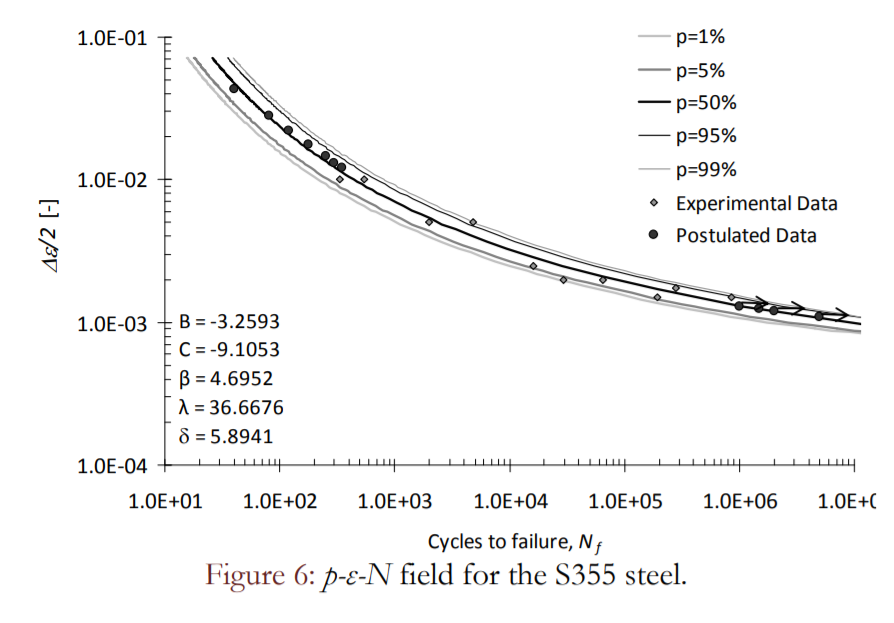
\includegraphics{images/p_e_n_paper.PNG}
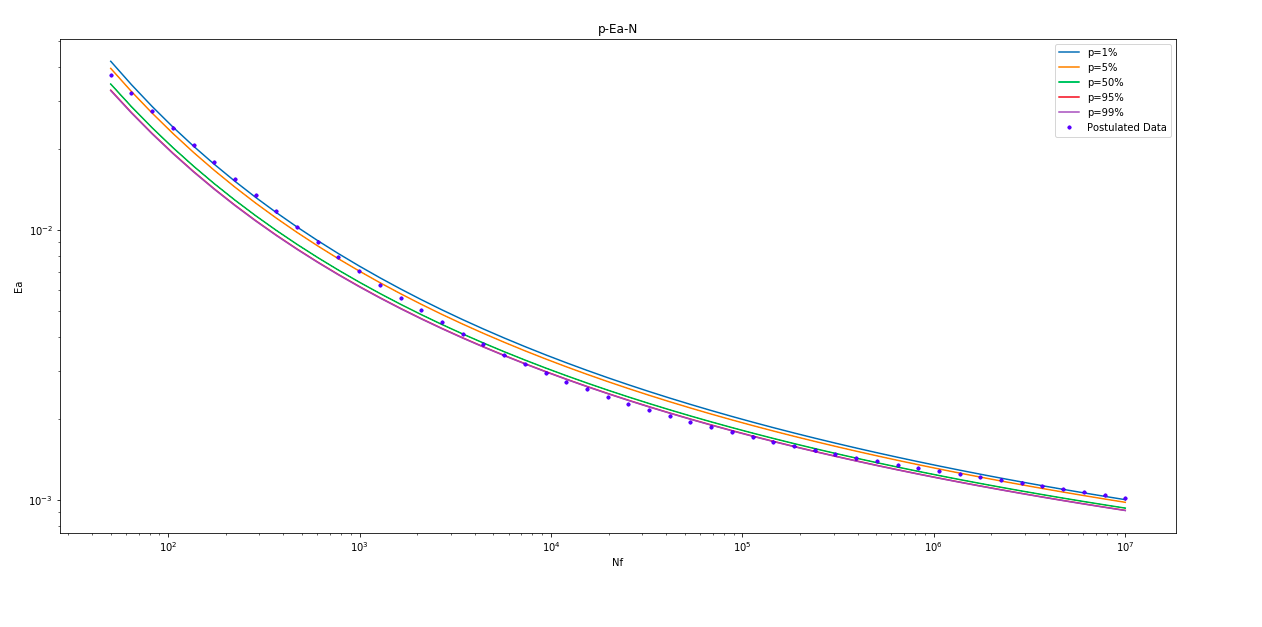
\includegraphics{images/p_e_n_model.PNG}

\textbf{The Above plots are for Strain vs Number of Cycles to Failure
for percent of probability along with postulated data (Experimental for
0.5 Percent).}

Comparison of results Probabilistic Shane Watson Damage Life Field:

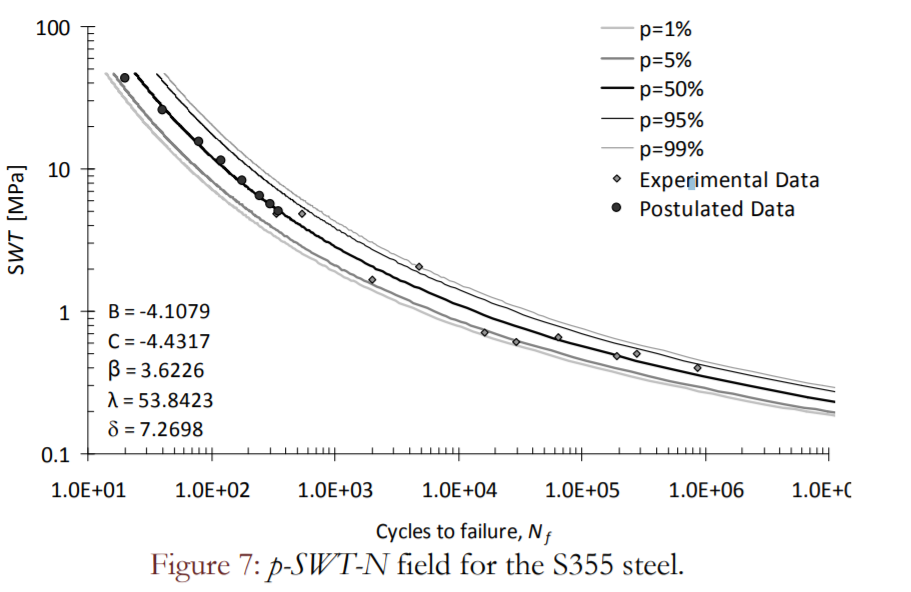
\includegraphics{images/p_s_n_paper.PNG}
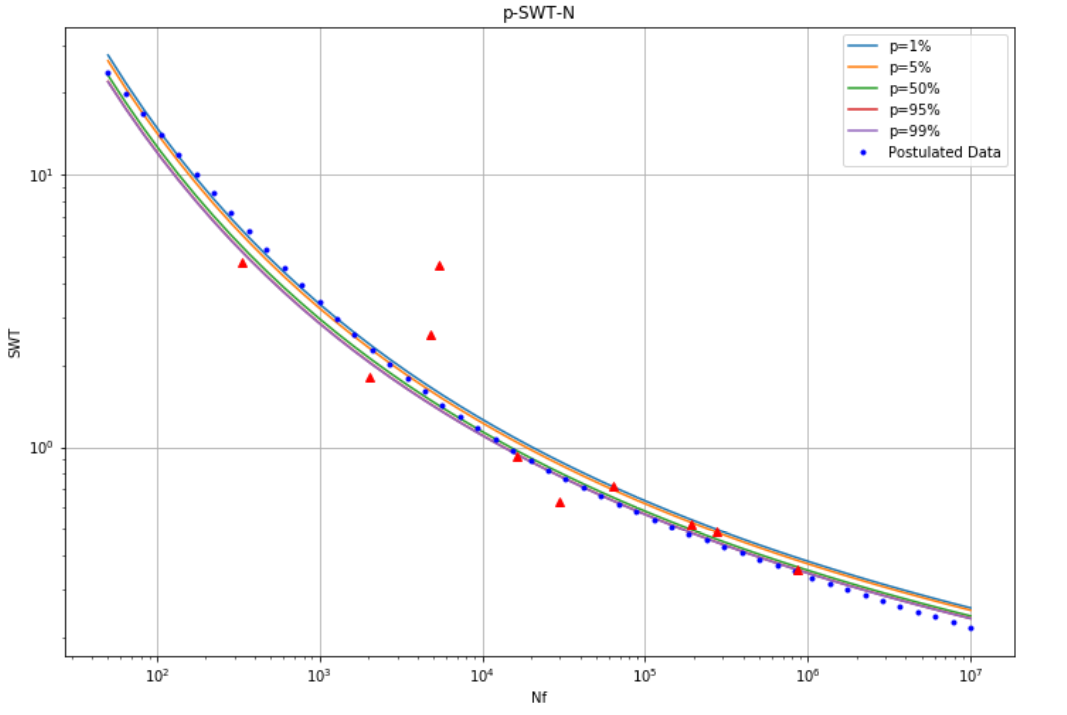
\includegraphics{images/p_s_n_model.PNG}

\textbf{The Above plots are for SWT Damage Parameter vs Number of Cycles
to Failure for percent of probability along with postulated data
(Experimental for 0.5 Percent).}

\hypertarget{new-work-done}{%
\subsubsection{5.3 New Work Done}\label{new-work-done}}

Estimating and supplying analysis of parameters assumed/supplied
externally and creating a closed form model with no external dependance
that computes probabilistic fatigue crack propogation data using only
the natural required input paramters.

\hypertarget{new-analysis}{%
\paragraph{5.3.1 New Analysis}\label{new-analysis}}

\begin{itemize}
\tightlist
\item
  To Estimate and Check if the SWT-N parameters can be predicted using
  gradient descent based regression.

  \begin{itemize}
  \tightlist
  \item
    Performance metric : To see if the Loss is reduced by Gradient
    descent or not and if the gradient descent works, if the predicted
    values match the supplied data.
  \end{itemize}
\item
  Estimate the parameters of Weibull Distribution using PWM estimation
  on real and predicted data.

  \begin{itemize}
  \tightlist
  \item
    Performance metric : To compare and see if the computed Weibull
    parameters using PWM match those supplied with the paper and if the
    predicted vs deterministic parameters match.
  \end{itemize}
\end{itemize}

\hypertarget{new-coding-algorithm}{%
\paragraph{5.3.2 New Coding / Algorithm}\label{new-coding-algorithm}}

\begin{itemize}
\tightlist
\item
  Coding and algorithm details here
\end{itemize}

\hypertarget{new-results}{%
\paragraph{5.3.3 New Results}\label{new-results}}

\begin{itemize}
\tightlist
\item
  Comparision of computed and given parameters.
\end{itemize}

\hypertarget{new-inferences}{%
\paragraph{5.3.4 New Inferences}\label{new-inferences}}

\begin{itemize}
\tightlist
\item
  Something like: parameter can be estimated using simple closed form
  coded solutions and shouldn't be estimated and or computed externally.
\end{itemize}

Students are advised to share the new derivations with results in
correlation with the reproduce results. Write clear inference for the
new results. You are also advised to add new analysis along with the
codes.

\hypertarget{inference-analysis-comparison}{%
\subsection{6 Inference Analysis/
Comparison}\label{inference-analysis-comparison}}

Add Stuff Here From Sir Arpitsinhs's Notebook.

\hypertarget{contribution-of-team-members}{%
\subsection{7 Contribution of team
members}\label{contribution-of-team-members}}

\hypertarget{technical-contribution-of-all-team-members}{%
\subsubsection{7.1 Technical contribution of all team
members}\label{technical-contribution-of-all-team-members}}

\hypertarget{non-technical-contribution-of-all-team-members}{%
\subsubsection{7.2 Non-Technical contribution of all team
members}\label{non-technical-contribution-of-all-team-members}}

\hypertarget{submission-checklist-for-uploading-on-google-drive}{%
\subsection{8 Submission checklist for uploading on Google
Drive}\label{submission-checklist-for-uploading-on-google-drive}}

This section provides the submission checklist for smooth and efficient
submission process. (This is for your reference and please remove this
while writing your report). - Soft copy of this project Report - Soft
copy of Abstract - Soft copy of Concept Map 1 and 2 - Soft copy of base
article - Soft copy of analysis (hand written)(jupyter notebooks) -
Folder of matlab(python) codes (with proper naming) - Folder of
reproduced results in .fig and .jpg format - latex (.tex) file of the
project report.

\begin{itemize}
\tightlist
\item
  {[}1{]} Noroozi, A.H., Glinka, G., Lambert, S., A two parameter
  driving force for fatigue crack growth analysis, International Journal
  of Fatigue, 27 (2005)1277-1296.
\item
  {[}2{]} Schütz, W., A History of Fatigue, Engineering Fracture
  Mechanics, 54 (1996) 263-300.
\item
  {[}3{]} Paris, P.C., Gomez, M., Anderson, W.E., A rational analytic
  theory of fatigue, Trend Engineering, 13 (1961) 9-14.
\item
  {[}4{]} Beden, S.M., Abdullah, S., Ariffin, A.K., Review of Fatigue
  Crack Propagation Models for Metallic Components, European Journal of
  Scientific Research, 28 (2009) 364-397.
\item
  {[}5{]} Coffin, L.F., A study of the effects of the cyclic thermal
  stresses on a ductile metal, Translations of the ASME, 76 (1954)
  931-950.
\item
  {[}6{]} Manson, S.S., Behaviour of materials under conditions of
  thermal stress, NACA TN-2933, National Advisory Committee for
  Aeronautics, (1954).
\item
  {[}7{]} Morrow, J.D., Cyclic plastic strain energy and fatigue of
  metals, Int. Friction, Damping and Cyclic Plasticity, ASTM STP 378,
  (1965) 45-87.
\item
  {[}8{]} Smith, K.N., Watson, P., Topper, T.H., A Stress-Strain
  Function for the Fatigue of Metals, Journal of Materials, 5(4) (1970)
  767-778.
\item
  {[}9{]} Shang, D.-G., Wang, D.-K., Li, M., Yao, W.-X., Local
  stress--strain field intensity approach to fatigue life prediction
  under random cyclic loading, International Journal of Fatigue, 23
  (2001) 903--910.
\item
  {[}10{]} Noroozi, A.H., Glinka, G., Lambert, S., A study of the stress
  ratio effects on fatigue crack growth using the unified two-parameter
  fatigue crack growth driving force, International Journal of Fatigue,
  29 (2007) 1616-1633.
\item
  {[}11{]} Noroozi, A.H., Glinka, G., Lambert, S., Prediction of fatigue
  crack growth under constant amplitude loading and a single overload
  based on elasto-plastic crack tip stresses and strains, Engineering
  Fracture Mechanics, 75 (2008) 188-206.
\item
  {[}12{]} Peeker, E., Niemi, E., Fatigue crack propagation model based
  on a local strain approach, Journal of Constructional Steel Research,
  49 (1999) 139--155.
\item
  {[}13{]} Glinka, G., A notch stress-strain analysis approach to
  fatigue crack growth, Engineering Fracture Mechanics, 21 (1985)
  245-261.
\item
  {[}14{]} Hurley, P.J., Evans, W.J., A methodology for predicting
  fatigue crack propagation rates in titanium based on damage
  accumulation, Scripta Materialia, 56 (2007) 681--684.
\item
  {[}15{]} Neuber, H., Theory of stress concentration for shear-strained
  prismatic bodies with arbitrary nonlinear stress--strain law, Trans.
  ASME Journal of Applied Mechanics, 28 (1961) 544--551.
\item
  {[}16{]} Moftakhar, A., Buczynski, A., Glinka, G., Calculation of
  elasto-plastic strains and stresses in notches under multiaxial
  loading, International Journal of Fracture, 70 (1995) 357-373.
\item
  {[}17{]} Reinhard, W., Moftakhar, A., Glinka, G., An Efficient Method
  for Calculating Multiaxial Elasto-Plastic Notch Tip Strains and
  Stresses under Proportional Loading, Fatigue and Fracture Mechanics,
  ASTM STP 1296, R.S. Piascik, J.C. Newman, N.E. Dowling, Eds., American
  Society for Testing and Materials, 27 (1997) 613-629.
\item
  {[}18{]} Mikheevskiy, S., Glinka, G., Elastic--plastic fatigue crack
  growth analysis under variable amplitude loading spectra,''
  International Journal of Fatigue, 31 (2009) 1828--1836.
\item
  {[}19{]} De Jesus, A.M.P., Matos, R., Fontoura, B.F.C., Rebelo, C.,
  Simões da Silva, L., Veljkovic, M., A comparison of the fatigue
  behavior between S355 and S690 steel grades, Journal of Constructional
  Steel Research, 79 (2012) 140--150.
\item
  {[}20{]} Castillo, E., Fernández-Canteli, A., A Unified Statistical
  Methodology for Modeling Fatigue Damage, Springer, (2009).
\item
  {[}21{]} Basquin, O.H., The exponential law of endurance tests, In:
  Proc. Annual Meeting, American Society for Testing Materials, 10
  (1910) 625-630.
\item
  {[}22{]} Creager, M., Paris, P.C., Elastic field equations for blunt
  cracks with reference to stress corrosion cracking, International
  Journal of Fracture Mechanics, 3 (1967) 247--252.
\item
  {[}23{]} Molski, K., Glinka, G., A method of elastic-plastic stress
  and strain calculation at a notch root, Materials Science and
  Engineering, 50 (1981) 93-100.
\item
  {[}24{]} Glinka, G., Development of weight functions and computer
  integration procedures for calculating stress intensity factors around
  cracks subjected to complex stress fields, Progress Report No.1:
  Stress and Fatigue-Fracture Design, Petersburg Ontario, Canada,
  (1996).
\item
  {[}25{]} Sadananda, K., Vasudevan, A.K., Kang, I.W., Effect of
  Superimposed Monotonic Fracture Modes on the ΔK and Kmax Parameters of
  Fatigue Crack Propagation, Acta Materialia, 51(22) (2003) 3399-3414.
\item
  {[}26{]} Kajawski, D., A new (ΔK+Kmax)0.5 driving force parameter for
  crack growth in aluminum alloys, International Journal of Fatigue,
  23(8) (2001) 733-740.
\item
  {[}27{]} Castillo, E., Galambos, J., Lifetime Regression Models Based
  on a Functional Equation of Physical Nature'', Journal of Applied
  Probability, 24 (1987) 160-169.
\item
  {[}28{]} Castillo, E., Fernández-Canteli, A., Hadi, A.S.,
  López-Anelle, M., A Fatigue Model with Local Sensitivity Analysis,
  Fatigue and Fracture of Engineering Material and Structure, 30 (2006)
  149--168.
\item
  {[}29{]}ASTM E606: Standard Practice for Strain-Controlled Fatigue
  Testing, Annual Book of ASTM Standards, ASTM, West Conshohocken, PA,
  USA, 03.01 (1998)
\item
  {[}30{]}ASTM E647: Standard Test Method for Measurement of Fatigue
  Crack Growth Rates, Annual Book of ASTM Standards, ASTM, West
  Conshohocken, PA, USA, 03.01 (2000).
\item
  {[}31{]} SAS, ANSYS, Swanson Analysis Systems, Inc., Houston, Version
  12.0, (2011).
\item
  {[}32{]} Ramberg, W., Osgood, W.R., Description of the stress-strain
  curves by the three parameters, NACA TN-902, National Advisory
  Committee for Aeronautics, (1943).
\end{itemize}

    \begin{tcolorbox}[breakable, size=fbox, boxrule=1pt, pad at break*=1mm,colback=cellbackground, colframe=cellborder]
\prompt{In}{incolor}{ }{\boxspacing}
\begin{Verbatim}[commandchars=\\\{\}]

\end{Verbatim}
\end{tcolorbox}


    % Add a bibliography block to the postdoc
    
    
    
\end{document}
